\documentclass{beamer}

\title{Formation KI} % Titre du rapport ou matière
\subtitle{LaTeX 2} % Sous-titre du rapport
\author{Yann Lapous (KI 025)}
\date{27 avril 2023}

\usepackage[utf8]{inputenc}
\usepackage[T1]{fontenc}
\usepackage[french]{babel}
\usepackage{svg}
\usepackage{tcolorbox}
\usepackage{xcolor}
\usepackage{listings}
\usepackage{appendix}
\usepackage{appendixnumberbeamer}
\usepackage{pgfplots}
\usepackage{qrcode}


\pgfplotsset{compat=1.18}

\usetheme{CambridgeUS}

% Définition de quelques couleurs (bleu du logo des Ponts)
\definecolor{bleuPonts}{HTML}{0194C6}

% Définition des couleurs du thème
\setbeamercolor{section in toc}{fg=black,bg=white}
\setbeamercolor{alerted text}{fg=red!80!gray}
\setbeamercolor*{palette primary}{fg=bleuPonts!60!black,bg=gray!30!white}
\setbeamercolor*{palette secondary}{fg=bleuPonts!70!black,bg=gray!15!white}
\setbeamercolor*{palette tertiary}{bg=bleuPonts!80!black,fg=gray!10!white}
\setbeamercolor*{palette quaternary}{fg=bleuPonts,bg=gray!5!white}

\setbeamercolor*{sidebar}{fg=red,bg=gray!15!white}
%set color structure
\setbeamercolor*{structure}{fg=bleuPonts!80!black}

\setbeamercolor*{palette sidebar primary}{fg=bleuPonts!10!black}
\setbeamercolor*{palette sidebar secondary}{fg=gray!10!blak}
\setbeamercolor*{palette sidebar tertiary}{fg=bleuPonts!50!black}
\setbeamercolor*{palette sidebar quaternary}{fg=gray!30!blak}

%\setbeamercolor*{titlelike}{parent=palette primary}
\setbeamercolor{titlelike}{parent=palette primary,fg=bleuPonts}
\setbeamercolor{frametitle}{bg=gray!10!white}
\setbeamercolor{frametitle right}{bg=gray!60!white}

\setbeamercolor*{separation line}{}
\setbeamercolor*{fine separation line}{}

% Définition de la page de garde
\defbeamertemplate*{title page}{customized}[1][]
{
    \centering
    \includesvg[width=0.2\paperwidth]{assets/logo.svg}\par
    \bigskip
    \usebeamerfont{title}\Huge{\inserttitle}\par
    \usebeamerfont{subtitle}\usebeamercolor[fg]{subtitle}\Large{\insertsubtitle}\par
}

% Définition de la forme des items
\setbeamertemplate{itemize items}[default]
\setbeamertemplate{enumerate items}[default]
\setbeamertemplate{section in toc}[square]

% Enlève la barre de navigation
\beamertemplatenavigationsymbolsempty

% Couleurs pour les listings (Dracula)
\definecolor{draculaBackground}{HTML}{282a36}
\definecolor{draculaCurentLine}{HTML}{44475a}
\definecolor{draculaSelection}{HTML}{44475a}
\definecolor{draculaForeground}{HTML}{f8f8f2}
\definecolor{draculaComment}{HTML}{6272a4}
\definecolor{draculaCyan}{HTML}{8be9fd}
\definecolor{draculaGreen}{HTML}{50fa7b}
\definecolor{draculaOrange}{HTML}{ffb86c}
\definecolor{draculaPink}{HTML}{ff79c6}
\definecolor{draculaPurple}{HTML}{bd93f9}
\definecolor{draculaRed}{HTML}{ff5555}
\definecolor{draculaYellow}{HTML}{f1fa8c}
%utilisation pour les listings de ces couleurs
% \lstset{
%     frame=tb,
%     basicstyle=\ttfamily\tiny\color{draculaForeground},
%     backgroundcolor=\color{draculaBackground},
%     commentstyle=\color{draculaComment},
%     keywordstyle=\color{draculaCyan},
%     stringstyle=\color{draculaGreen},
%     identifierstyle=\color{draculaPink},
%     breaklines=true,
%     numbers=left,
%     numberstyle=\color{bleuPonts},
%     extendedchars=true,
%     xleftmargin=5mm,
%     xrightmargin=5mm
% }

\definecolor{codegreen}{rgb}{0,0.6,0}
\definecolor{codegray}{rgb}{0.5,0.5,0.5}
\definecolor{codepurple}{rgb}{0.58,0,0.82}
\definecolor{backcolour}{rgb}{0.95,0.95,0.92}

\lstdefinestyle{mystyle}{
    backgroundcolor=\color{backcolour},   
    commentstyle=\color{codegreen},
    keywordstyle=\color{magenta},
    numberstyle=\tiny\color{codegray},
    stringstyle=\color{codepurple},
    identifierstyle=\color{blue},
    basicstyle=\ttfamily\footnotesize,
    breakatwhitespace=false,         
    breaklines=true,                 
    captionpos=b,                    
    keepspaces=true,                 
    numbers=left,                    
    numbersep=5pt,                  
    showspaces=false,                
    showstringspaces=false,
    showtabs=false,                  
    tabsize=2
}

\lstset{style=mystyle}

\begin{document}
    \begin{frame}
        \titlepage
    \end{frame}

    \begin{frame}
        \frametitle{Sommaire}
        \setcounter{tocdepth}{1}
        \tableofcontents
    \end{frame}
    \section*{Introduction}
    \begin{frame}
        \frametitle{Introduction}
        \centering
        
\includegraphics[width=.5\textwidth]{assets/image1.png}
    \end{frame}
    \section{Implémenter du code}
    \subsection{Commandes}
    \begin{frame} [allowframebreaks=1,fragile,t]
        \begin{lstlisting}[language=python]
            def hello_world():
                print("Hello World")
            if __name__ == "__main__":
                hello_world()
        \end{lstlisting}
        \begin{block}{Comment afficher ?}
            il faut utiliser le package \texttt{listings}, \lstinline[language=tex]!\usepackage{listings}!
            \begin{itemize}
            \item \lstinline[language=tex]{\lstinline[language=python]!print("Hello World")!} 
            \item \lstinline[language=tex]!\lstinline[language=python]{print("Hello World")}!
            \item \lstinline[language=tex]!\begin{lstlisting}[language=python] ... \end{lstlisting}!
            \item \lstinline[language=tex]!\lstinputlisting[language=python]{main.py}!
            \end{itemize}
        \end{block}
    \end{frame}
    \subsection{Customiser la mise en forme}
    \begin{frame}
        \frametitle{Imposer un style}
        \lstinputlisting[language=tex]{assets/code_1.tex}
        \begin{alertblock}{Attention}
            Ici il faut définir les couleurs grace au package \texttt{xcolor}
        \end{alertblock}
    \end{frame}
    \begin{frame}[allowframebreaks=1,fragile,t]
        \frametitle{Créer un style}
        \lstinputlisting[language=tex]{assets/code_2.tex}
        \begin{block}{Utilisation}
            \lstinline[language=tex]!\lstset{style=mystyle}!
        \end{block}
    \end{frame}

    \section{Ajouter des graphiques et des figures}
    \subsection{Images}
    \begin{frame}
        \centering
        \includesvg[width=0.2\paperwidth]{assets/enpc.svg}
        \begin{block}{\texttt{includesvg} et \texttt{includegraphics}}
            \lstinputlisting[language=tex]{assets/code_3.tex}
        \end{block}
    \end{frame}
    \subsection{Graphiques}
    \begin{frame}
        \frametitle{Graphiques PNG}
        \begin{figure}[H]
            \centering
            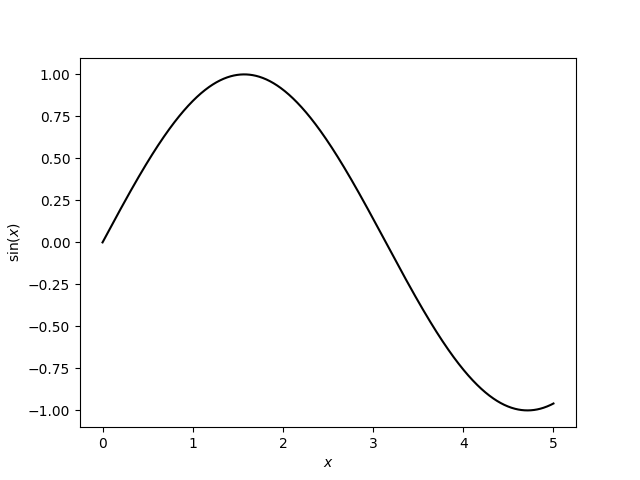
\includegraphics[width=8cm,height=6cm]{assets/graphique.png}
            \caption{Graphique png}
        \end{figure}
    \end{frame}
    \begin{frame}
        \frametitle{Graphiques PGF}
        \begin{figure}[H]
        \centering
            % This file was created with tikzplotlib v0.10.1.
\begin{tikzpicture}

\definecolor{darkgray176}{RGB}{176,176,176}

\begin{axis}[
height=6cm,
tick align=outside,
tick pos=left,
width=8cm,
x grid style={darkgray176},
xlabel={\(\displaystyle x\)},
xmin=-0.25, xmax=5.25,
xtick style={color=black},
y grid style={darkgray176},
ylabel={\(\displaystyle \sin(x)\)},
ymin=-1.09999714523008, ymax=1.09999954924673,
ytick style={color=black}
]
\addplot [semithick, black]
table {%
0 0
0.005005005005005 0.00500498410907264
0.01001001001001 0.0100098428431792
0.015015015015015 0.0150144508304942
0.02002002002002 0.0200186827054735
0.025025025025025 0.0250224131119944
0.03003003003003 0.0300255167064961
0.035035035035035 0.0350278681611196
0.04004004004004 0.0400293421668466
0.045045045045045 0.0450298134366394
0.05005005005005 0.0500291567085786
0.0550550550550551 0.0550272467490012
0.0600600600600601 0.0600239583556376
0.0650650650650651 0.0650191663607483
0.0700700700700701 0.0700127456342586
0.0750750750750751 0.0750045710868939
0.0800800800800801 0.0799945176733128
0.0850850850850851 0.0849824603952395
0.0900900900900901 0.089968274304595
0.0950950950950951 0.0949518345066271
0.1001001001001 0.0999330161630392
0.105105105105105 0.104911694495117
0.11011011011011 0.109887744786855
0.115115115115115 0.11486104238808
0.12012012012012 0.119831462717573
0.125125125125125 0.124798881266192
0.13013013013013 0.129763173599989
0.135135135135135 0.134724215363328
0.14014014014014 0.139681882281999
0.145145145145145 0.144636050166333
0.15015015015015 0.149586594914311
0.155155155155155 0.154533392514675
0.16016016016016 0.159476319050032
0.165165165165165 0.16441525069996
0.17017017017017 0.169350063744107
0.175175175175175 0.174280634565295
0.18018018018018 0.179206839652612
0.185185185185185 0.184128555604509
0.19019019019019 0.189045659131888
0.195195195195195 0.193958027061194
0.2002002002002 0.198865536337499
0.205205205205205 0.203768064027582
0.21021021021021 0.208665487323014
0.215215215215215 0.213557683543229
0.22022022022022 0.218444530138601
0.225225225225225 0.223325904693511
0.23023023023023 0.228201684929414
0.235235235235235 0.233071748707905
0.24024024024024 0.237935974033775
0.245245245245245 0.242794239058069
0.25025025025025 0.247646422081136
0.255255255255255 0.252492401555682
0.26026026026026 0.257332056089811
0.265265265265265 0.262165264450065
0.27027027027027 0.266991905564465
0.275275275275275 0.271811858525541
0.28028028028028 0.276625002593361
0.285285285285285 0.281431217198558
0.29029029029029 0.286230381945345
0.295295295295295 0.291022376614535
0.3003003003003 0.295807081166554
0.305305305305305 0.300584375744443
0.31031031031031 0.305354140676863
0.315315315315315 0.310116256481096
0.32032032032032 0.31487060386603
0.325325325325325 0.319617063735156
0.33033033033033 0.324355517189545
0.335335335335335 0.329085845530831
0.34034034034034 0.333807930264181
0.345345345345345 0.338521653101264
0.35035035035035 0.343226895963216
0.355355355355355 0.347923540983595
0.36036036036036 0.352611470511338
0.365365365365365 0.357290567113702
0.37037037037037 0.36196071357921
0.375375375375375 0.366621792920588
0.38038038038038 0.371273688377692
0.385385385385385 0.375916283420433
0.39039039039039 0.380549461751701
0.395395395395395 0.385173107310272
0.4004004004004 0.389787104273721
0.405405405405405 0.394391337061317
0.41041041041041 0.398985690336924
0.415415415415415 0.403570049011888
0.42042042042042 0.40814429824792
0.425425425425425 0.412708323459972
0.43043043043043 0.417262010319109
0.435435435435435 0.421805244755369
0.44044044044044 0.426337912960628
0.445445445445445 0.430859901391444
0.45045045045045 0.435371096771903
0.455455455455455 0.439871386096457
0.46046046046046 0.444360656632758
0.465465465465465 0.448838795924474
0.47047047047047 0.453305691794116
0.475475475475475 0.457761232345839
0.48048048048048 0.462205305968252
0.485485485485485 0.466637801337208
0.49049049049049 0.471058607418597
0.495495495495495 0.475467613471127
0.500500500500501 0.479864709049094
0.505505505505506 0.484249784005156
0.510510510510511 0.488622728493083
0.515515515515516 0.492983432970517
0.520520520520521 0.497331788201711
0.525525525525526 0.501667685260267
0.530530530530531 0.505991015531866
0.535535535535536 0.510301670716985
0.540540540540541 0.514599542833614
0.545545545545546 0.518884524219957
0.550550550550551 0.523156507537134
0.555555555555556 0.527415385771866
0.560560560560561 0.531661052239154
0.565565565565566 0.535893400584958
0.570570570570571 0.540112324788854
0.575575575575576 0.544317719166695
0.580580580580581 0.548509478373257
0.585585585585586 0.552687497404875
0.590590590590591 0.556851671602077
0.595595595595596 0.561001896652205
0.600600600600601 0.565138068592027
0.605605605605606 0.569260083810341
0.610610610610611 0.573367839050571
0.615615615615616 0.577461231413356
0.620620620620621 0.581540158359124
0.625625625625626 0.58560451771066
0.630630630630631 0.589654207655672
0.635635635635636 0.593689126749333
0.640640640640641 0.597709173916828
0.645645645645646 0.601714248455884
0.650650650650651 0.605704250039292
0.655655655655656 0.609679078717422
0.660660660660661 0.613638634920724
0.665665665665666 0.617582819462226
0.670670670670671 0.621511533540014
0.675675675675676 0.625424678739712
0.680680680680681 0.629322157036943
0.685685685685686 0.633203870799786
0.690690690690691 0.637069722791224
0.695695695695696 0.640919616171576
0.700700700700701 0.644753454500924
0.705705705705706 0.648571141741532
0.710710710710711 0.652372582260246
0.715715715715716 0.656157680830896
0.720720720720721 0.659926342636675
0.725725725725726 0.663678473272519
0.730730730730731 0.667413978747471
0.735735735735736 0.671132765487032
0.740740740740741 0.674834740335512
0.745745745745746 0.678519810558354
0.750750750750751 0.682187883844466
0.755755755755756 0.685838868308528
0.760760760760761 0.689472672493297
0.765765765765766 0.693089205371894
0.770770770770771 0.696688376350088
0.775775775775776 0.700270095268565
0.780780780780781 0.703834272405184
0.785785785785786 0.707380818477226
0.790790790790791 0.710909644643631
0.795795795795796 0.714420662507224
0.800800800800801 0.717913784116926
0.805805805805806 0.721388921969962
0.810810810810811 0.724845989014049
0.815815815815816 0.728284898649579
0.820820820820821 0.731705564731787
0.825825825825826 0.73510790157291
0.830830830830831 0.738491823944332
0.835835835835836 0.741857247078721
0.840840840840841 0.74520408667215
0.845845845845846 0.748532258886212
0.850850850850851 0.751841680350116
0.855855855855856 0.755132268162779
0.860860860860861 0.758403939894902
0.865865865865866 0.761656613591032
0.870870870870871 0.76489020777162
0.875875875875876 0.768104641435059
0.880880880880881 0.77129983405971
0.885885885885886 0.774475705605926
0.890890890890891 0.777632176518052
0.895895895895896 0.780769167726421
0.900900900900901 0.78388660064933
0.905905905905906 0.786984397195014
0.910910910910911 0.790062479763599
0.915915915915916 0.793120771249046
0.920920920920921 0.796159195041084
0.925925925925926 0.799177675027127
0.930930930930931 0.802176135594183
0.935935935935936 0.805154501630746
0.940940940940941 0.80811269852868
0.945945945945946 0.811050652185084
0.950950950950951 0.813968289004153
0.955955955955956 0.816865535899017
0.960960960960961 0.819742320293575
0.965965965965966 0.822598570124314
0.970970970970971 0.825434213842109
0.975975975975976 0.828249180414021
0.980980980980981 0.831043399325073
0.985985985985986 0.833816800580017
0.990990990990991 0.836569314705089
0.995995995995996 0.839300872749747
1.001001001001 0.842011406288401
1.00600600600601 0.844700847422122
1.01101101101101 0.847369128780349
1.01601601601602 0.850016183522573
1.02102102102102 0.852641945340013
1.02602602602603 0.855246348457276
1.03103103103103 0.857829327634003
1.03603603603604 0.860390818166507
1.04104104104104 0.862930755889393
1.04604604604605 0.865449077177161
1.05105105105105 0.867945718945808
1.05605605605606 0.870420618654399
1.06106106106106 0.87287371430664
1.06606606606607 0.875304944452428
1.07107107107107 0.877714248189395
1.07607607607608 0.880101565164426
1.08108108108108 0.882466835575175
1.08608608608609 0.884810000171567
1.09109109109109 0.887131000257273
1.0960960960961 0.889429777691189
1.1011011011011 0.891706274888888
1.10610610610611 0.893960434824063
1.11111111111111 0.896192201029956
1.11611611611612 0.898401517600773
1.12112112112112 0.900588329193084
1.12612612612613 0.902752581027207
1.13113113113113 0.904894218888586
1.13613613613614 0.907013189129143
1.14114114114114 0.909109438668625
1.14614614614615 0.911182914995934
1.15115115115115 0.913233566170439
1.15615615615616 0.915261340823283
1.16116116116116 0.917266188158664
1.16616616616617 0.919248057955111
1.17117117117117 0.92120690056674
1.17617617617618 0.923142666924499
1.18118118118118 0.925055308537396
1.18618618618619 0.926944777493716
1.19119119119119 0.928811026462217
1.1961961961962 0.930654008693322
1.2012012012012 0.932473678020282
1.20620620620621 0.934269988860341
1.21121121121121 0.936042896215869
1.21621621621622 0.937792355675498
1.22122122122122 0.939518323415228
1.22622622622623 0.941220756199528
1.23123123123123 0.942899611382418
1.23623623623624 0.944554846908538
1.24124124124124 0.946186421314198
1.24624624624625 0.947794293728425
1.25125125125125 0.949378423873976
1.25625625625626 0.950938772068355
1.26126126126126 0.952475299224806
1.26626626626627 0.953987966853286
1.27127127127127 0.955476737061439
1.27627627627628 0.956941572555535
1.28128128128128 0.958382436641414
1.28628628628629 0.959799293225395
1.29129129129129 0.96119210681519
1.2962962962963 0.962560842520787
1.3013013013013 0.963905466055324
1.30630630630631 0.965225943735952
1.31131131131131 0.966522242484675
1.31631631631632 0.967794329829179
1.32132132132132 0.969042173903647
1.32632632632633 0.970265743449557
1.33133133133133 0.971465007816464
1.33633633633634 0.972639936962768
1.34134134134134 0.973790501456467
1.34634634634635 0.974916672475894
1.35135135135135 0.97601842181044
1.35635635635636 0.977095721861258
1.36136136136136 0.978148545641959
1.36636636636637 0.979176866779281
1.37137137137137 0.980180659513758
1.37637637637638 0.981159898700357
1.38138138138138 0.982114559809117
1.38638638638639 0.983044618925752
1.39139139139139 0.983950052752263
1.3963963963964 0.98483083860751
1.4014014014014 0.985686954427788
1.40640640640641 0.986518378767376
1.41141141141141 0.987325090799075
1.41641641641642 0.988107070314731
1.42142142142142 0.988864297725739
1.42642642642643 0.989596754063535
1.43143143143143 0.990304420980071
1.43643643643644 0.990987280748274
1.44144144144144 0.991645316262493
1.44644644644645 0.992278511038921
1.45145145145145 0.992886849216016
1.45645645645646 0.993470315554893
1.46146146146146 0.994028895439706
1.46646646646647 0.994562574878016
1.47147147147147 0.995071340501142
1.47647647647648 0.995555179564492
1.48148148148148 0.996014079947888
1.48648648648649 0.996448030155864
1.49149149149149 0.996857019317958
1.4964964964965 0.997241037188981
1.5015015015015 0.997600074149278
1.50650650650651 0.997934121204964
1.51151151151151 0.998243169988153
1.51651651651652 0.998527212757166
1.52152152152152 0.998786242396725
1.52652652652653 0.999020252418132
1.53153153153153 0.99922923695943
1.53653653653654 0.999413190785551
1.54154154154154 0.999572109288449
1.54654654654655 0.999705988487211
1.55155155155155 0.99981482502816
1.55655655655656 0.999898616184939
1.56156156156156 0.999957359858576
1.56656656656657 0.999991054577542
1.57157157157157 0.999999699497783
1.57657657657658 0.999983294402744
1.58158158158158 0.999941839703372
1.58658658658659 0.999875336438109
1.59159159159159 0.999783786272863
1.5965965965966 0.999667191500968
1.6016016016016 0.999525555043125
1.60660660660661 0.999358880447331
1.61161161161161 0.999167171888789
1.61661661661662 0.998950434169802
1.62162162162162 0.998708672719655
1.62662662662663 0.998441893594478
1.63163163163163 0.998150103477094
1.63663663663664 0.997833309676852
1.64164164164164 0.997491520129444
1.64664664664665 0.997124743396706
1.65165165165165 0.996732988666404
1.65665665665666 0.996316265752002
1.66166166166166 0.995874585092419
1.66666666666667 0.995407957751765
1.67167167167167 0.994916395419067
1.67667667667668 0.994399910407971
1.68168168168168 0.993858515656439
1.68668668668669 0.993292224726422
1.69169169169169 0.992701051803521
1.6966966966967 0.992085011696631
1.7017017017017 0.99144411983757
1.70670670670671 0.990778392280694
1.71171171171171 0.990087845702494
1.71671671671672 0.989372497401178
1.72172172172172 0.988632365296235
1.72672672672673 0.987867467927994
1.73173173173173 0.98707782445715
1.73673673673674 0.986263454664289
1.74174174174174 0.985424378949395
1.74674674674675 0.984560618331332
1.75175175175175 0.983672194447325
1.75675675675676 0.982759129552411
1.76176176176176 0.981821446518887
1.76676676676677 0.980859168835734
1.77177177177177 0.979872320608031
1.77677677677678 0.978860926556347
1.78178178178178 0.977825012016127
1.78678678678679 0.976764602937054
1.79179179179179 0.9756797258824
1.7967967967968 0.974570408028359
1.8018018018018 0.973436677163368
1.80680680680681 0.972278561687413
1.81181181181181 0.971096090611312
1.81681681681682 0.969889293555992
1.82182182182182 0.968658200751747
1.82682682682683 0.967402843037481
1.83183183183183 0.966123251859931
1.83683683683684 0.964819459272888
1.84184184184184 0.963491497936384
1.84684684684685 0.962139401115881
1.85185185185185 0.960763202681436
1.85685685685686 0.959362937106851
1.86186186186186 0.95793863946881
1.86686686686687 0.956490345446002
1.87187187187187 0.955018091318225
1.87687687687688 0.953521913965478
1.88188188188188 0.952001850867038
1.88688688688689 0.950457940100521
1.89189189189189 0.948890220340927
1.8968968968969 0.94729873085967
1.9019019019019 0.9456835115236
1.90690690690691 0.944044602793997
1.91191191191191 0.942382045725562
1.91691691691692 0.940695881965387
1.92192192192192 0.938986153751915
1.92692692692693 0.937252903913874
1.93193193193193 0.935496175869213
1.93693693693694 0.933716013624011
1.94194194194194 0.93191246177137
1.94694694694695 0.930085565490308
1.95195195195195 0.928235370544616
1.95695695695696 0.926361923281721
1.96196196196196 0.924465270631519
1.96696696696697 0.922545460105203
1.97197197197197 0.92060253979407
1.97697697697698 0.918636558368318
1.98198198198198 0.916647565075827
1.98698698698699 0.914635609740923
1.99199199199199 0.912600742763135
1.996996996997 0.910543015115926
2.002002002002 0.90846247834542
2.00700700700701 0.906359184569112
2.01201201201201 0.904233186474558
2.01701701701702 0.902084537318059
2.02202202202202 0.899913290923325
2.02702702702703 0.897719501680129
2.03203203203203 0.895503224542941
2.03703703703704 0.893264515029553
2.04204204204204 0.891003429219689
2.04704704704705 0.888720023753603
2.05205205205205 0.886414355830651
2.05705705705706 0.884086483207868
2.06206206206206 0.881736464198517
2.06706706706707 0.879364357670626
2.07207207207207 0.87697022304552
2.07707707707708 0.874554120296325
2.08208208208208 0.872116109946469
2.08708708708709 0.869656253068168
2.09209209209209 0.867174611280892
2.0970970970971 0.864671246749825
2.1021021021021 0.862146222184306
2.10710710710711 0.859599600836258
2.11211211211211 0.857031446498602
2.11711711711712 0.854441823503665
2.12212212212212 0.851830796721561
2.12712712712713 0.84919843155857
2.13213213213213 0.8465447939555
2.13713713713714 0.843869950386034
2.14214214214214 0.841173967855064
2.14714714714715 0.838456913897013
2.15215215215215 0.835718856574146
2.15715715715716 0.832959864474861
2.16216216216216 0.830180006711972
2.16716716716717 0.82737935292098
2.17217217217217 0.824557973258327
2.17717717717718 0.821715938399638
2.18218218218218 0.818853319537949
2.18718718718719 0.81597018838193
2.19219219219219 0.813066617154081
2.1971971971972 0.810142678588929
2.2022022022022 0.807198445931199
2.20720720720721 0.804233992933989
2.21221221221221 0.801249393856913
2.21721721721722 0.798244723464245
2.22222222222222 0.795220057023049
2.22722722722723 0.792175470301287
2.23223223223223 0.789111039565926
2.23723723723724 0.786026841581025
2.24224224224224 0.782922953605816
2.24724724724725 0.779799453392761
2.25225225225225 0.776656419185614
2.25725725725726 0.773493929717452
2.26226226226226 0.770312064208709
2.26726726726727 0.767110902365188
2.27227227227227 0.763890524376066
2.27727727727728 0.760651010911886
2.28228228228228 0.757392443122534
2.28728728728729 0.754114902635207
2.29229229229229 0.750818471552369
2.2972972972973 0.747503232449694
2.3023023023023 0.744169268373998
2.30730730730731 0.740816662841155
2.31231231231231 0.737445499834012
2.31731731731732 0.734055863800278
2.32232232232232 0.730647839650414
2.32732732732733 0.727221512755502
2.33233233233233 0.723776968945109
2.33733733733734 0.720314294505136
2.34234234234234 0.716833576175656
2.34734734734735 0.713334901148744
2.35235235235235 0.709818357066289
2.35735735735736 0.706284032017799
2.36236236236236 0.702732014538199
2.36736736736737 0.699162393605606
2.37237237237237 0.695575258639107
2.37737737737738 0.691970699496515
2.38238238238238 0.688348806472117
2.38738738738739 0.684709670294418
2.39239239239239 0.681053382123861
2.3973973973974 0.677380033550548
2.4024024024024 0.673689716591946
2.40740740740741 0.669982523690577
2.41241241241241 0.666258547711708
2.41741741741742 0.662517881941024
2.42242242242242 0.658760620082286
2.42742742742743 0.65498685625499
2.43243243243243 0.651196684992006
2.43743743743744 0.647390201237211
2.44244244244244 0.643567500343109
2.44744744744745 0.639728678068444
2.45245245245245 0.635873830575803
2.45745745745746 0.632003054429204
2.46246246246246 0.628116446591676
2.46746746746747 0.624214104422835
2.47247247247247 0.620296125676441
2.47747747747748 0.616362608497951
2.48248248248248 0.612413651422061
2.48748748748749 0.608449353370234
2.49249249249249 0.604469813648228
2.4974974974975 0.600475131943603
2.5025025025025 0.596465408323227
2.50750750750751 0.592440743230769
2.51251251251251 0.58840123748418
2.51751751751752 0.584346992273173
2.52252252252252 0.580278109156681
2.52752752752753 0.576194690060319
2.53253253253253 0.57209683727383
2.53753753753754 0.567984653448519
2.54254254254254 0.563858241594684
2.54754754754755 0.559717705079037
2.55255255255255 0.555563147622112
2.55755755755756 0.551394673295667
2.56256256256256 0.54721238652008
2.56756756756757 0.54301639206173
2.57257257257257 0.538806795030374
2.57757757757758 0.534583700876513
2.58258258258258 0.530347215388752
2.58758758758759 0.52609744469115
2.59259259259259 0.521834495240559
2.5975975975976 0.51755847382396
2.6026026026026 0.513269487555788
2.60760760760761 0.508967643875246
2.61261261261261 0.504653050543616
2.61761761761762 0.500325815641559
2.62262262262262 0.49598604756641
2.62762762762763 0.491633855029456
2.63263263263263 0.487269347053221
2.63763763763764 0.482892632968729
2.64264264264264 0.478503822412767
2.64764764764765 0.474103025325139
2.65265265265265 0.469690351945915
2.65765765765766 0.465265912812661
2.66266266266266 0.460829818757679
2.66766766766767 0.456382180905227
2.67267267267267 0.451923110668734
2.67767767767768 0.447452719748011
2.68268268268268 0.442971120126453
2.68768768768769 0.438478424068233
2.69269269269269 0.433974744115489
2.6976976976977 0.429460193085507
2.7027027027027 0.424934884067893
2.70770770770771 0.420398930421741
2.71271271271271 0.415852445772794
2.71771771771772 0.411295544010595
2.72272272272272 0.406728339285638
2.72772772772773 0.402150946006505
2.73273273273273 0.397563478837002
2.73773773773774 0.392966052693287
2.74274274274274 0.38835878274099
2.74774774774775 0.383741784392326
2.75275275275275 0.379115173303212
2.75775775775776 0.374479065370359
2.76276276276276 0.369833576728378
2.76776776776777 0.365178823746865
2.77277277277277 0.360514923027487
2.77777777777778 0.355841991401066
2.78278278278278 0.351160145924643
2.78778778778779 0.346469503878556
2.79279279279279 0.341770182763495
2.7977977977978 0.33706230029756
2.8028028028028 0.332345974413315
2.80780780780781 0.327621323254831
2.81281281281281 0.322888465174727
2.81781781781782 0.318147518731206
2.82282282282282 0.313398602685084
2.82782782782783 0.308641835996817
2.83283283283283 0.303877337823519
2.83783783783784 0.299105227515978
2.84284284284284 0.294325624615665
2.84784784784785 0.289538648851743
2.85285285285285 0.284744420138063
2.85785785785786 0.279943058570164
2.86286286286286 0.275134684422264
2.86786786786787 0.270319418144243
2.87287287287287 0.265497380358632
2.87787787787788 0.260668691857588
2.88288288288288 0.255833473599867
2.88788788788789 0.250991846707798
2.89289289289289 0.246143932464244
2.8978978978979 0.241289852309567
2.9029029029029 0.236429727838587
2.90790790790791 0.231563680797533
2.91291291291291 0.226691833080992
2.91791791791792 0.221814306728863
2.92292292292292 0.216931223923291
2.92792792792793 0.212042706985612
2.93293293293293 0.207148878373287
2.93793793793794 0.202249860676834
2.94294294294294 0.197345776616757
2.94794794794795 0.192436749040476
2.95295295295295 0.187522900919242
2.95795795795796 0.182604355345063
2.96296296296296 0.177681235527618
2.96796796796797 0.17275366479117
2.97297297297297 0.167821766571479
2.97797797797798 0.162885664412708
2.98298298298298 0.157945481964328
2.98798798798799 0.153001342978023
2.99299299299299 0.148053371304586
2.997997997998 0.143101690890821
3.003003003003 0.138146425776436
3.00800800800801 0.133187700090934
3.01301301301301 0.128225638050507
3.01801801801802 0.123260363954922
3.02302302302302 0.118292002184409
3.02802802802803 0.113320677196544
3.03303303303303 0.108346513523129
3.03803803803804 0.10336963576708
3.04304304304304 0.0983901685992976
3.04804804804805 0.0934082367555474
3.05305305305305 0.088423965033336
3.05805805805806 0.0834374782887838
3.06306306306306 0.0784489014334974
3.06806806806807 0.0734583594314408
3.07307307307307 0.068465977295805
3.07807807807808 0.0634718800858764
3.08308308308308 0.058476192903904
3.08808808808809 0.0534790408919656
3.09309309309309 0.0484805492288331
3.0980980980981 0.0434808431268367
3.1031031031031 0.0384800478287283
3.10810810810811 0.0334782886045441
3.11311311311311 0.0284756907484667
3.11811811811812 0.0234723795756867
3.12312312312312 0.0184684804192629
3.12812812812813 0.0134641186269834
3.13313313313313 0.00845941955822523
3.13813813813814 0.00345450858081416
3.14314314314314 -0.00155048893211566
3.14814814814815 -0.00655544760526236
3.15315315315315 -0.011560242064297
3.15815815815816 -0.0165647469390043
3.16316316316316 -0.021568836866423
3.16816816816817 -0.0265723864939862
3.17317317317317 -0.0315752704826617
3.17817817817818 -0.0365773635100914
3.18318318318318 -0.041578540273731
3.18818818818819 -0.0465786754939883
3.19319319319319 -0.0515776439173622
3.1981981981982 -0.0565753203195796
3.2032032032032 -0.0615715795087325
3.20820820820821 -0.0665662963284149
3.21321321321321 -0.0715593456608556
3.21821821821822 -0.0765506024300554
3.22322322322322 -0.0815399416049184
3.22822822822823 -0.0865272382023843
3.23323323323323 -0.0915123672905598
3.23823823823824 -0.0964952039918475
3.24324324324324 -0.101475623486074
3.24824824824825 -0.106453501013618
3.25325325325325 -0.111428711878534
3.25825825825826 -0.116401131451675
3.26326326326326 -0.121370635173819
3.26826826826827 -0.126337098558784
3.27327327327327 -0.131300397196548
3.27827827827828 -0.136260406756368
3.28328328328328 -0.14121700298989
3.28828828828829 -0.146170061734267
3.29329329329329 -0.151119458915264
3.2982982982983 -0.156065070550368
3.3033033033033 -0.161006772751895
3.30830830830831 -0.165944441730092
3.31331331331331 -0.17087795379624
3.31831831831832 -0.175807185365747
3.32332332332332 -0.180732012961251
3.32832832832833 -0.185652313215708
3.33333333333333 -0.190567962875485
3.33833833833834 -0.195478838803446
3.34334334334334 -0.200384817982036
3.34834834834835 -0.205285777516365
3.35335335335335 -0.210181594637285
3.35835835835836 -0.215072146704466
3.36336336336336 -0.219957311209466
3.36836836836837 -0.224836965778804
3.37337337337337 -0.229710988177021
3.37837837837838 -0.234579256309744
3.38338338338338 -0.239441648226747
3.38838838838839 -0.244298042125001
3.39339339339339 -0.249148316351728
3.3983983983984 -0.253992349407447
3.4034034034034 -0.258830019949021
3.40840840840841 -0.263661206792691
3.41341341341341 -0.268485788917118
3.41841841841842 -0.273303645466409
3.42342342342342 -0.278114655753147
3.42842842842843 -0.282918699261416
3.43343343343343 -0.287715655649815
3.43843843843844 -0.292505404754478
3.44344344344344 -0.297287826592081
3.44844844844845 -0.302062801362846
3.45345345345345 -0.306830209453549
3.45845845845846 -0.311589931440506
3.46346346346346 -0.316341848092574
3.46846846846847 -0.321085840374132
3.47347347347347 -0.325821789448065
3.47847847847848 -0.330549576678742
3.48348348348348 -0.335269083634983
3.48848848848849 -0.339980192093032
3.49349349349349 -0.344682784039516
3.4984984984985 -0.349376741674397
3.5035035035035 -0.354061947413931
3.50850850850851 -0.358738283893607
3.51351351351351 -0.36340563397109
3.51851851851852 -0.368063880729152
3.52352352352352 -0.372712907478608
3.52852852852853 -0.377352597761231
3.53353353353353 -0.381982835352673
3.53853853853854 -0.386603504265377
3.54354354354354 -0.391214488751482
3.54854854854855 -0.39581567330572
3.55355355355355 -0.400406942668315
3.55855855855856 -0.404988181827863
3.56356356356356 -0.409559276024219
3.56856856856857 -0.41412011075137
3.57357357357357 -0.418670571760302
3.57857857857858 -0.423210545061861
3.58358358358358 -0.427739916929614
3.58858858858859 -0.432258573902693
3.59359359359359 -0.436766402788636
3.5985985985986 -0.441263290666227
3.6036036036036 -0.445749124888323
3.60860860860861 -0.450223793084674
3.61361361361361 -0.45468718316474
3.61861861861862 -0.459139183320496
3.62362362362362 -0.463579682029239
3.62862862862863 -0.468008568056373
3.63363363363363 -0.472425730458203
3.63863863863864 -0.47683105858471
3.64364364364364 -0.481224442082324
3.64864864864865 -0.485605770896688
3.65365365365365 -0.489974935275416
3.65865865865866 -0.494331825770839
3.66366366366366 -0.498676333242752
3.66866866866867 -0.503008348861144
3.67367367367367 -0.507327764108924
3.67867867867868 -0.511634470784642
3.68368368368368 -0.515928361005198
3.68868868868869 -0.520209327208543
3.69369369369369 -0.524477262156376
3.6986986986987 -0.528732058936831
3.7037037037037 -0.532973610967149
3.70870870870871 -0.537201811996357
3.71371371371371 -0.541416556107922
3.71871871871872 -0.545617737722407
3.72372372372372 -0.549805251600119
3.72872872872873 -0.553978992843737
3.73373373373373 -0.55813885690095
3.73873873873874 -0.562284739567068
3.74374374374374 -0.566416536987635
3.74874874874875 -0.570534145661031
3.75375375375375 -0.574637462441066
3.75875875875876 -0.57872638453956
3.76376376376376 -0.582800809528922
3.76876876876877 -0.586860635344713
3.77377377377377 -0.590905760288204
3.77877877877878 -0.594936083028921
3.78378378378378 -0.59895150260719
3.78878878878879 -0.602951918436658
3.79379379379379 -0.606937230306816
3.7987987987988 -0.610907338385512
3.8038038038038 -0.614862143221449
3.80880880880881 -0.618801545746673
3.81381381381381 -0.622725447279064
3.81881881881882 -0.626633749524796
3.82382382382382 -0.630526354580811
3.82882882882883 -0.634403164937263
3.83383383383383 -0.638264083479963
3.83883883883884 -0.642109013492815
3.84384384384384 -0.645937858660233
3.84884884884885 -0.64975052306956
3.85385385385385 -0.653546911213464
3.85885885885886 -0.657326927992336
3.86386386386386 -0.66109047871667
3.86886886886887 -0.664837469109434
3.87387387387387 -0.668567805308433
3.87887887887888 -0.67228139386866
3.88388388388388 -0.675978141764638
3.88888888888889 -0.679657956392746
3.89389389389389 -0.683320745573545
3.8988988988989 -0.686966417554083
3.9039039039039 -0.690594881010193
3.90890890890891 -0.694206045048782
3.91391391391391 -0.697799819210109
3.91891891891892 -0.701376113470049
3.92392392392392 -0.704934838242351
3.92892892892893 -0.708475904380876
3.93393393393393 -0.711999223181837
3.93893893893894 -0.715504706386018
3.94394394394394 -0.718992266180986
3.94894894894895 -0.722461815203286
3.95395395395395 -0.725913266540638
3.95895895895896 -0.729346533734107
3.96396396396396 -0.73276153078027
3.96896896896897 -0.736158172133375
3.97397397397397 -0.739536372707477
3.97897897897898 -0.742896047878576
3.98398398398398 -0.746237113486732
3.98898898898899 -0.749559485838174
3.99399399399399 -0.7528630817074
3.998998998999 -0.756147818339259
4.004004004004 -0.759413613451022
4.00900900900901 -0.762660385234447
4.01401401401401 -0.765888052357827
4.01901901901902 -0.769096533968027
4.02402402402402 -0.77228574969251
4.02902902902903 -0.775455619641348
4.03403403403403 -0.778606064409228
4.03903903903904 -0.781737005077437
4.04404404404404 -0.784848363215838
4.04904904904905 -0.78794006088484
4.05405405405405 -0.791012020637345
4.05905905905906 -0.794064165520692
4.06406406406406 -0.797096419078582
4.06906906906907 -0.800108705352993
4.07407407407407 -0.803100948886087
4.07907907907908 -0.806073074722094
4.08408408408408 -0.809025008409194
4.08908908908909 -0.811956676001381
4.09409409409409 -0.814868004060316
4.0990990990991 -0.817758919657163
4.1041041041041 -0.820629350374421
4.10910910910911 -0.823479224307736
4.11411411411411 -0.8263084700677
4.11911911911912 -0.829117016781642
4.12412412412412 -0.831904794095403
4.12912912912913 -0.834671732175098
4.13413413413413 -0.837417761708866
4.13913913913914 -0.840142813908602
4.14414414414414 -0.842846820511688
4.14914914914915 -0.845529713782696
4.15415415415415 -0.84819142651509
4.15915915915916 -0.850831892032904
4.16416416416416 -0.853451044192416
4.16916916916917 -0.856048817383806
4.17417417417417 -0.858625146532796
4.17917917917918 -0.861179967102282
4.18418418418418 -0.86371321509395
4.18918918918919 -0.86622482704988
4.19419419419419 -0.868714740054136
4.1991991991992 -0.87118289173434
4.2042042042042 -0.873629220263236
4.20920920920921 -0.876053664360239
4.21421421421421 -0.878456163292968
4.21921921921922 -0.880836656878772
4.22422422422422 -0.88319508548623
4.22922922922923 -0.885531390036653
4.23423423423423 -0.887845512005558
4.23923923923924 -0.890137393424138
4.24424424424424 -0.89240697688071
4.24924924924925 -0.894654205522157
4.25425425425425 -0.896879023055351
4.25925925925926 -0.899081373748561
4.26426426426426 -0.901261202432853
4.26926926926927 -0.903418454503467
4.27427427427427 -0.905553075921192
4.27927927927928 -0.90766501321371
4.28428428428428 -0.909754213476946
4.28928928928929 -0.911820624376384
4.29429429429429 -0.913864194148385
4.2992992992993 -0.915884871601479
4.3043043043043 -0.91788260611765
4.30930930930931 -0.919857347653602
4.31431431431431 -0.921809046742016
4.31931931931932 -0.923737654492784
4.32432432432432 -0.925643122594239
4.32932932932933 -0.927525403314361
4.33433433433433 -0.929384449501974
4.33933933933934 -0.931220214587931
4.34434434434434 -0.933032652586272
4.34934934934935 -0.934821718095386
4.35435435435435 -0.93658736629914
4.35935935935936 -0.938329552968006
4.36436436436436 -0.94004823446017
4.36936936936937 -0.941743367722619
4.37437437437437 -0.943414910292228
4.37937937937938 -0.945062820296817
4.38438438438438 -0.946687056456202
4.38938938938939 -0.948287578083231
4.39439439439439 -0.9498643450848
4.3993993993994 -0.95141731796286
4.4044044044044 -0.952946457815406
4.40940940940941 -0.954451726337449
4.41441441441441 -0.955933085821977
4.41941941941942 -0.957390499160903
4.42442442442442 -0.958823929845989
4.42942942942943 -0.960233341969764
4.43443443443443 -0.961618700226421
4.43943943943944 -0.962979969912704
4.44444444444444 -0.964317116928778
4.44944944944945 -0.965630107779079
4.45445445445445 -0.966918909573156
4.45945945945946 -0.968183490026494
4.46446446446446 -0.969423817461325
4.46946946946947 -0.970639860807418
4.47447447447447 -0.971831589602859
4.47947947947948 -0.972998973994816
4.48448448448448 -0.974141984740281
4.48948948948949 -0.975260593206811
4.49449449449449 -0.976354771373237
4.4994994994995 -0.977424491830372
4.5045045045045 -0.978469727781693
4.50950950950951 -0.979490453044016
4.51451451451451 -0.98048664204815
4.51951951951952 -0.981458269839538
4.52452452452452 -0.982405312078882
4.52952952952953 -0.983327745042751
4.53453453453453 -0.984225545624179
4.53953953953954 -0.985098691333241
4.54454454454454 -0.985947160297618
4.54954954954955 -0.986770931263141
4.55455455455455 -0.98756998359433
4.55955955955956 -0.988344297274905
4.56456456456456 -0.989093852908291
4.56956956956957 -0.989818631718103
4.57457457457457 -0.990518615548615
4.57957957957958 -0.991193786865215
4.58458458458458 -0.991844128754847
4.58958958958959 -0.992469624926432
4.59459459459459 -0.993070259711276
4.5995995995996 -0.993646018063465
4.6046046046046 -0.994196885560238
4.60960960960961 -0.994722848402352
4.61461461461461 -0.995223893414426
4.61961961961962 -0.995700008045271
4.62462462462462 -0.996151180368205
4.62962962962963 -0.99657739908135
4.63463463463463 -0.996978653507918
4.63963963963964 -0.997354933596477
4.64464464464464 -0.997706229921202
4.64964964964965 -0.998032533682111
4.65465465465465 -0.998333836705288
4.65965965965966 -0.998610131443086
4.66466466466466 -0.998861410974315
4.66966966966967 -0.999087669004418
4.67467467467467 -0.999288899865624
4.67967967967968 -0.999465098517097
4.68468468468468 -0.999616260545057
4.68968968968969 -0.99974238216289
4.69469469469469 -0.999843460211248
4.6996996996997 -0.999919492158124
4.7047047047047 -0.999970476098915
4.70970970970971 -0.999996410756472
4.71471471471471 -0.999997295481132
4.71971971971972 -0.999973130250732
4.72472472472472 -0.999923915670612
4.72972972972973 -0.999849652973599
4.73473473473473 -0.999750344019973
4.73973973973974 -0.999625991297428
4.74474474474474 -0.999476597921001
4.74974974974975 -0.999302167633001
4.75475475475475 -0.999102704802909
4.75975975975976 -0.998878214427274
4.76476476476476 -0.998628702129586
4.76976976976977 -0.998354174160132
4.77477477477477 -0.998054637395845
4.77977977977978 -0.997730099340128
4.78478478478478 -0.997380568122666
4.78978978978979 -0.997006052499225
4.79479479479479 -0.996606561851428
4.7997997997998 -0.996182106186527
4.8048048048048 -0.995732696137145
4.80980980980981 -0.995258342961014
4.81481481481481 -0.994759058540692
4.81981981981982 -0.994234855383265
4.82482482482482 -0.993685746620034
4.82982982982983 -0.993111746006186
4.83483483483483 -0.99251286792045
4.83983983983984 -0.991889127364736
4.84484484484484 -0.991240539963758
4.84984984984985 -0.990567121964646
4.85485485485485 -0.989868890236535
4.85985985985986 -0.989145862270148
4.86486486486486 -0.98839805617735
4.86986986986987 -0.987625490690701
4.87487487487487 -0.986828185162985
4.87987987987988 -0.986006159566723
4.88488488488488 -0.985159434493675
4.88988988988989 -0.984288031154323
4.89489489489489 -0.983391971377342
4.8998998998999 -0.982471277609048
4.9049049049049 -0.981525972912842
4.90990990990991 -0.980556080968628
4.91491491491491 -0.979561626072221
4.91991991991992 -0.978542633134739
4.92492492492492 -0.977499127681979
4.92992992992993 -0.976431135853775
4.93493493493493 -0.975338684403348
4.93993993993994 -0.974221800696631
4.94494494494494 -0.973080512711586
4.94994994994995 -0.971914849037504
4.95495495495495 -0.970724838874287
4.95995995995996 -0.969510512031715
4.96496496496496 -0.968271898928704
4.96996996996997 -0.967009030592541
4.97497497497497 -0.965721938658106
4.97997997997998 -0.964410655367081
4.98498498498498 -0.963075213567143
4.98998998998999 -0.96171564671114
4.99499499499499 -0.960331988856251
5 -0.958924274663138
};
\end{axis}

\end{tikzpicture}
 
            \caption{Graphique pgf}
        \end{figure}
    \end{frame}
    \begin{frame}
        \begin{block}{Meilleure solution}
            La meilleure solution : utiliser Python pour faire ses
            graphiques grace aux packages \texttt{matplotlib} et \texttt{tikzplotlib}
        \end{block}
        \begin{block}{Dans Python}
            \lstinline[language=python]{tikzplotlib.save("nom_du_fichier.tex")}
        \end{block}
        \begin{block}{Dans LaTeX}
            \lstinputlisting[language=tex]{assets/code_4.tex}
        \end{block}
    \end{frame}
    \section{Ajouter une bibliographie}
    \begin{frame}
        \frametitle{Fichier \texttt{.bib}}
        \lstinputlisting[language=tex]{assets/code_bib.bib}
    \end{frame}
    \begin{frame}
        \frametitle{Utilisation}
        \lstinputlisting[language=tex]{assets/code_bibtex.tex}
    \end{frame}
    \begin{frame}
        \frametitle{Zotero}
        \begin{columns}
        \column{0.8\textwidth}
            \centering
            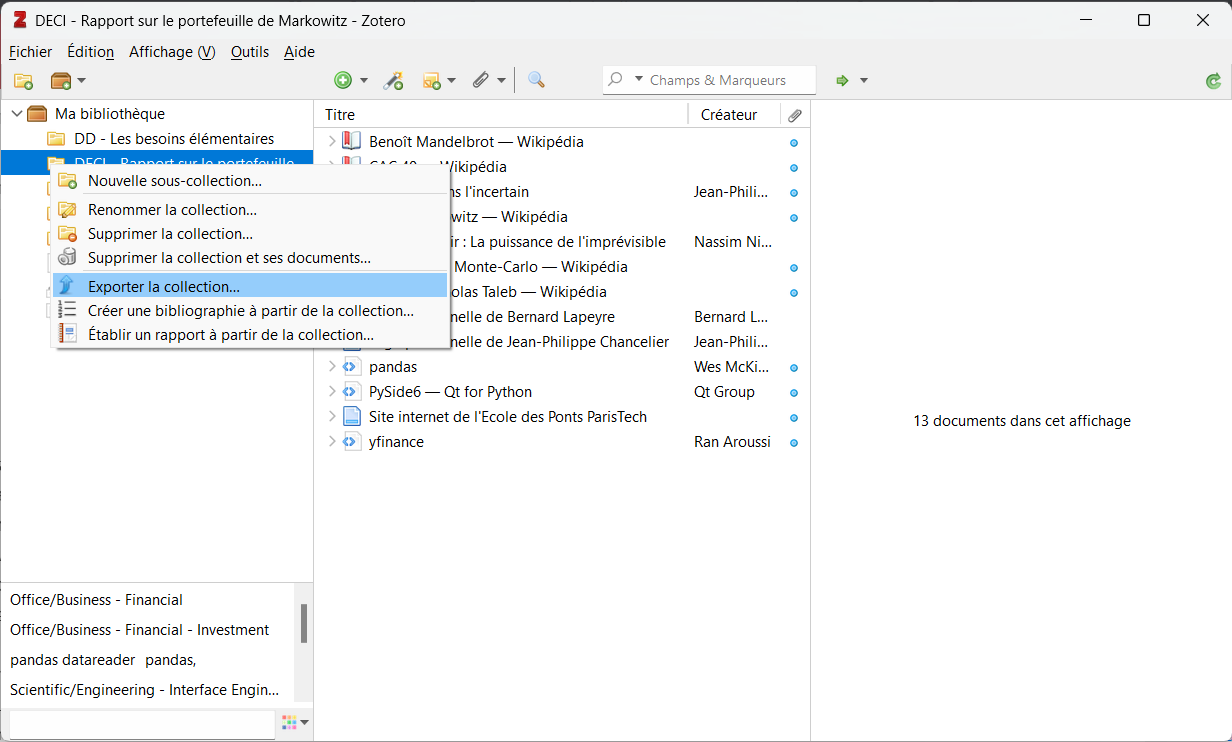
\includegraphics[width=1\textwidth]{assets/zotero.png}
        \column{0.2\textwidth}
            \centering
            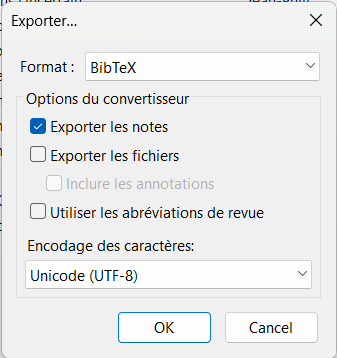
\includegraphics[width=1\textwidth]{assets/zotero2.png}
        \end{columns}
    \end{frame}
    \section{Faire des présentations}
    \begin{frame}
        \frametitle{Beamer}
        \begin{block}{Beamer}
            Beamer est un package LaTeX qui permet de faire des présentations
        \end{block}
        \centering
        \Huge{Vous savez déjà faire !}
    \end{frame}
    \begin{frame}
        \frametitle{Exemple}
        \begin{alertblock}{Particularité}
            Contrairement à la classse \texttt{article}, il faut utiliser les environnements \texttt{frame} pour
            préciser à \LaTeX{} où commencent et où finissent les diapositives.
        \end{alertblock}

        \lstinputlisting[language=tex]{assets/code_beamer.tex}
    \end{frame}
    \section*{Conclusion}
    \begin{frame}
        \centering
        \Huge Merci, à vous de jouer !
        
        \vspace{1cm}

        \normalsize\url{https://kiclubinfo.notion.site/Formation-LaTeX-2-e1fd51c463754565876d215aaf670ce0}

        \vspace{.5cm}
        \qrcode[height=.3\textwidth]{https://kiclubinfo.notion.site/Formation-LaTeX-2-e1fd51c463754565876d215aaf670ce0}
    \end{frame}

\end{document}
